\documentclass[a4paper,12pt,twoside]{article}
\usepackage[left=1in,right=1in,top=1in,bottom=1in]{geometry}

\usepackage{xeCJK}
\setCJKmainfont{Songti TC}
\setCJKfamilyfont{kai}{Songti TC}
\newcommand{\kai}{\CJKfamily{kai}} % 用 \kai{使用楷書}

\usepackage{lmodern}
\usepackage{titling}
\usepackage{titlesec}
\usepackage{graphicx}
\usepackage{float}
\usepackage{amsmath, amsthm, amssymb, amsfonts, mathrsfs}
\usepackage{upgreek} % 直立的希臘字母

\usepackage[shortlabels]{enumitem}
\usepackage{setspace}
\renewcommand{\baselinestretch}{1.5}
\usepackage[colorlinks]{hyperref}
\usepackage{fancyvrb}
\usepackage{fancyhdr}
\usepackage{multicol}
\usepackage{caption}
\usepackage{listings}
\usepackage{bm}
\usepackage{bbm} % for \mathbbm{1} (indicator function)
\usepackage{centernot}
\usepackage{mdframed}
\usepackage{tikz}
\usetikzlibrary{patterns, arrows.meta, positioning}
\usepackage[nameinlink, capitalise]{cleveref}
\usepackage{diagbox}
\usepackage{booktabs}
\usepackage{multirow,array}
\usepackage{tabularx}
\usepackage{mathtools}
\usepackage{indentfirst} % 首段 indent
\setlength{\parindent}{2em}
\usepackage{cancel} % 數學式子畫線槓掉
\newcommand\mcancel[2][red]{\setbox0=\hbox{$#2$}%
\rlap{\raisebox{.45\ht0}{\textcolor{#1}{\rule{\wd0}{1pt}}}}#2}
\usepackage{datetime2}

\AtBeginDocument{%
 \setlength{\abovedisplayskip}{6pt}
 \setlength{\belowdisplayskip}{6pt}
 \setlength{\abovedisplayshortskip}{4pt}
 \setlength{\belowdisplayshortskip}{4pt}
}

\definecolor{codegreen}{rgb}{0,0.6,0}
\definecolor{codegray}{rgb}{0.5,0.5,0.5}
\definecolor{codepurple}{rgb}{0.58,0,0.82}
\definecolor{backcolour}{rgb}{0.95,0.95,0.92}

\lstdefinestyle{mystyle}{
 backgroundcolor=\color{backcolour},
 commentstyle=\color{codegreen},
 keywordstyle=\color{magenta},
 numberstyle=\tiny\color{codegray},
 stringstyle=\color{codepurple},
 basicstyle=\ttfamily\footnotesize,
 breakatwhitespace=false,
 breaklines=true,
 captionpos=b,
 keepspaces=true,
 numbers=left,
 numbersep=5pt,
 showspaces=false,
 showstringspaces=false,
 showtabs=false,
 tabsize=2
}
\lstset{style=mystyle}

\hypersetup{citecolor=blue, linkcolor=blue, urlcolor=blue}

\DeclareMathOperator{\supp}{supp}
\DeclareMathOperator{\skewness}{Skewness}
\DeclareMathOperator{\DU}{D-U}
\DeclareMathOperator{\CU}{C-U}
\DeclareMathOperator{\Geo}{Geo}
\DeclareMathOperator{\Pois}{Pois}
\DeclareMathOperator{\Gam}{Gam}
\DeclareMathOperator{\LN}{LogN}
\DeclareMathOperator{\cov}{Cov}
\DeclareMathOperator*{\argmax}{arg\,max}
\DeclareMathOperator*{\argmin}{arg\,min}
\DeclareMathOperator{\re}{Re}
\DeclareMathOperator{\im}{Im}

\newcommand{\N}{\mathbb{N}}
\newcommand{\Z}{\mathbb{Z}}
\newcommand{\Q}{\mathbb{Q}}
\newcommand{\R}{\mathbb{R}}
\newcommand{\C}{\mathbb{C}}
\newcommand{\G}{\mathcal{G}}
\newcommand{\mP}{\mathbb{P}}
\newcommand{\F}{\mathcal{F}}
\newcommand{\B}{\mathcal{B}}
\newcommand{\1}{\mathbbm{1}}
\newcommand{\Poi}{\text{Poi}}
\newcommand{\Var}{\text{Var}}
\newcommand{\as}{\text{a.s.}}
\newcommand{\vect}[1]{\boldsymbol{\mathbf{#1}}}
\newcommand{\paren}[1]{\left({#1}\right)}
\newcommand{\brk}[1]{\left[{#1}\right]}
\newcommand{\curl}[1]{\left\{{#1}\right\}}
\renewcommand{\lambda}{\lambdaup}

\theoremstyle{definition} % 定理環境 style 改用正體
\newtheorem{theorem}{定理}
\newtheorem{definition}{定義}
\newtheorem*{definition*}{定義}
\newtheorem{example}{例子}
\newtheorem{exercise}{練習}
\newtheorem{corollary}{推論}
\newtheorem{property}{性質}
\newtheorem{prop}{命題}
\newtheorem{lemma}{引理}
\newtheorem{problem}{問題}
\newtheorem*{remark}{註}

\renewcommand{\figurename}{圖}
\renewcommand{\tablename}{表}

\DeclareMathOperator{\var}{Var}
\DeclareMathOperator{\corr}{corr}
\DeclareMathOperator{\rank}{rank}
\DeclareMathOperator{\MSE}{MSE}
\DeclareMathOperator{\SSE}{SSE}
\DeclareMathOperator{\SST}{SST}
\DeclareMathOperator{\SSR}{SSR}
\DeclareMathOperator{\sgn}{sign}
\DeclareMathOperator{\alt}{Alt}
\DeclareMathOperator{\adj}{adj}
\DeclareMathOperator{\curlOp}{curl}
\DeclareMathOperator{\spn}{span}
\DeclareMathOperator{\sse}{SSE}
\DeclareMathOperator{\tr}{tr}

\newcommand{\ep}{\varepsilon}
\newcommand{\p}{\partial}
\newcommand{\abs}[1]{\left|#1\right|}
\newcommand\norm[1]{\left\lVert#1\right\rVert}
\newcommand{\innerprod}[1]{\langle#1\rangle}
\newcommand{\ds}{\displaystyle}
\newcommand{\blank}{\rule[-1mm]{1.5cm}{0.1mm}}
\newcommand{\dint}{\displaystyle\int}
\renewcommand{\bar}{\overline}

\newtheoremstyle{remark}{}{}{}{}{\bfseries\sffamily}{.}{.5em}{#1}
\theoremstyle{remark}

\newtheorem*{remark*}{\textit{Remark}}
\newtheorem*{solution*}{解}

\AtEndEnvironment{solution*}{\hfill$\square$}
\newtheorem*{hint*}{Hint}


\newcommand{\redtext}[1]{{\color{red} #1}}
\newcommand{\bluetext}[1]{{\color{blue} #1}}

\fancypagestyle{firstpage}{
  \fancyhf{}
  \fancyhead[R]{\small《高中數學實驗教材》第 2 冊}
  \fancyhead[L]{\small 第 4 章\quad 指數函數與對數函數}
  \fancyfoot[C]{\thepage}
}

\pagestyle{fancy}
\setlength{\headheight}{14pt}
\renewcommand{\headrulewidth}{0.5pt}
\renewcommand{\footrulewidth}{0pt}
\fancyhead{}
\fancyhead[LE]{\small 《高中數學實驗教材》第二冊}
\fancyhead[RO]{\small 第四章\quad 指數函數與對數函數}
\fancyfoot[C]{\thepage}

\title{\LARGE\textbf{《高中數學實驗教材》第二冊}\\[0.5em] \Large\textbf{第四章\quad 指數函數與對數函數}}
\author{\textbf{高中數學實驗教材編輯小組}\quad 編著}
\date{民國六十二年（1973）初版}

\begin{document}

\maketitle
\thispagestyle{firstpage}

% ==========================================
% 掃描檔勘誤、文字校訂與疑難處說明（依規則整理於目錄之前）
% ==========================================
\section*{【說明】掃描檔勘誤、疑難處與文義校訂表}
\addcontentsline{toc}{section}{【說明】掃描檔勘誤、疑難處與文義校訂表}
\label{sec:errata_notes}

本章依據 1973 年版《高中數學實驗教材 第二冊》（高一下）第四章「指數函數與對數函數」掃描原件轉錄為 \LaTeX{} 格式。為忠實反映教材原始內容並兼顧排版品質與嚴謹性，依作業規範將掃描檔中出現之印刷訛誤、符號缺漏、字模損毀、歷史印記雜訊及文義疑難處詳細考證彙整於下表。讀者可點擊表格中之章節連結直接跳至正文對應位置：

\begin{table}[H]
\centering
\small
\renewcommand{\arraystretch}{1.35}
\begin{tabularx}{\textwidth}{|p{3.2cm}|p{3.6cm}|X|}
\hline
\textbf{章節位置} & \textbf{掃描檔原始現象 / 誤植} & \textbf{考證說明與校訂處理} \\ \hline

\hyperref[note:b2-ch4-p81-duplicate]{§ 1-1 頁 81 【例】(ii)} & 
「$(a^{-3})^2 = (1/a^3)^2 = \frac{1}{(a^3)^2} = \frac{1}{(a^3)^2} = 1/a^6$」 & 
算式中「$\frac{1}{(a^3)^2}$」重複排印兩次，係鉛字排版之重植贅墨。正文忠實保留原刊印文字，特予考證備註。 \\ \hline

\hyperref[note:b2-ch4-p81-comma]{§ 1-1 頁 81 習題 4-1 第 2 題} & 
「$(a, b)^n = a^n \cdot b^n$」 & 
乘積運算符號誤植為逗號（或鉛字點號浮墨），文義顯係 $(a\cdot b)^n$ 或 $(ab)^n$。正文照原刊印字樣錄入並在此說明。 \\ \hline

\hyperref[note:b2-ch4-p91-monotonicity]{§ 2 頁 91 單調性「注意」段} & 
「$\alpha > \beta \implies g(\alpha) \le g(\beta)$ 叫做單調遞增」及「$\alpha < \beta \implies g(\alpha) \ge g(\beta)$ 叫做單調遞減」 & 
不等號方向排印倒置（非嚴格遞增應為 $\alpha > \beta \implies g(\alpha) \ge g(\beta)$，遞減應為 $\le$）。正文忠實保留原書排印文字，特予說明。 \\ \hline

\hyperref[note:b2-ch4-p92-missing-f]{§ 2 頁 92 定理 2 證明 (i) 第 6 行} & 
「$f(0)\cdot f(\beta) = (0+\beta) = f(\beta)$」 & 
中間等式脫漏函數記號 $f$（漏印為 $(0+\beta)$），文義實為 $f(0+\beta)$。正文忠實照錄原印文字並在此備註。 \\ \hline

\hyperref[note:b2-ch4-p98-log-base]{§ 3-2 頁 98 習題 4-5 第 1(v) 題} & 
「$\log 1000^{\frac{1}{10}}$」 & 
同題其他小題皆標明底數（如 $\log_5, \log_3$ 等），此小題脫漏底數標籤 10（即常用對數 $\log_{10}$）。正文忠實照錄原印字樣。 \\ \hline

\hyperref[note:b2-ch4-p106-surjcetion]{§ 4-1 頁 106 蓋射定義} & 
「蓋射 (surjcetion)」 & 
英文術語拼寫字母倒置誤植為「surjcetion」（正確為 surjection）。正文維持原書鉛字排印並在此考釋。 \\ \hline

\hyperref[note:b2-ch4-p109-index-x]{§ 4-2 頁 109 定理 7 證明第 11 行} & 
「$x_n < a_1 < x_0,\; x = 1, 2, 3, \dots$」 & 
式中變數符號 $x$ 顯為數列指標符號 $n$ 之誤植（應為 $n = 1, 2, 3, \dots$）。正文照錄原書文字並予備註說明。 \\ \hline

\end{tabularx}
\end{table}

\clearpage
\tableofcontents
\newpage

% =========================================================================
% 《高中數學實驗教材》第二冊（高一下） 
% 第四章 指數函數與對數函數
% =========================================================================

\section{指數函數與對數函數}\label{sec:b2_ch4}

對於每一個正實數 $a$，我們用 $a^n$ 表示 $n$ 個相乘的連乘積. 例如：
\[
a^1 = a,\quad a^2 = a\cdot a,\quad a^3 = a\cdot a\cdot a,\quad \dots\dots\dots\dots,
\]
\[
a^{n+1} = a^n \cdot a,\quad \dots\dots \text{等}.
\]
所以指數符號 $a^n$ 只是 $a$ 自乘 $n$ 次的簡寫，而下列大家所熟悉的指數定則乃是乘法結合律的一個直接推論：
\begin{align}
a^n \cdot a^m &= a^{n+m} \label{eq:b2-ch4-intro-exp-rule-1} \\
(a^n)^m &= a^{nm} \label{eq:b2-ch4-intro-exp-rule-2}
\end{align}

在本章第一節中，我們將討論如何把指數的定義逐步推廣到負整數指數，分數指數及實數指數，使得推廣後的廣義指數符號 $a^\alpha\; (\alpha \in \mathbb{R})$ 依然滿足指數定則：
\begin{align}
a^\alpha \cdot a^\beta &= a^{\alpha+\beta} \label{eq:b2-ch4-intro-gen-rule-1} \\
(a^\alpha)^\beta &= a^{\alpha\beta} \label{eq:b2-ch4-intro-gen-rule-2}
\end{align}
當我們將指數的範圍推廣到全實數系後，$a^\alpha$ 中的 $\alpha$ 可以在實數系 $\mathbb{R}$ 中任意變更皆有明確的意義. 所以 $y = a^x$ 是一個函數（參看第一冊第五章 § 3）. 我們把它叫做指數函數. 我們將在 § 2 中討論指數函數的重要特性，在 § 3 中討論指數函數的反函數——對數函數——及它的性質. 指數函數與對數函數是研究許多自然現象及社會問題的重要工具.

\subsection{指數定則與指數定義的推廣}\label{sec:b2_4-1}

\subsubsection*{1-1 負整數指數的定義}

首先，我們要把指數的定義推廣到全整數系 $\mathbb{Z}$.

\begin{definition*}
對於正實數 $a$，我們定義 $a^0 = 1,\; a^{-n} = \frac{1}{a^n},\; n \in \mathbb{N}$.
\end{definition*}

\noindent\textbf{【討論】} 假想我們所定義的 $a^0$ 和 $a^{-n}$ 依然滿足指數定則，那麼由下列計算可以看出 $a^0$ 必須等於 1，$a^{-n}$ 必須等於 $\frac{1}{a^n}$，這就是我們如此定義 $a^0$ 和 $a^{-n}$ 的原因：\\
因
\[
a^0 \cdot a^n = a^{0+n} = a^n, \quad \text{但是 } a^n \neq 0, \text{ 所以 } a^0 = 1.
\]
又
\[
a^{-n} \cdot a^n = a^{-n+n} = a^0 = 1, \quad \text{所以 } a^{-n} = \frac{1}{a^n}.
\]
同學們應該注意：上面所談的並不是 $a^0 = 1$ 的證明，因為在 $a^0$ 根本還沒有定義前，要去證明它等於什麼數是完全沒有意義的. 同學們也許要問，$a^0$ 可不可以定義成其他的數呢？例如定義
\[
a^0 = 2,
\]
自然也沒有關係，但是這樣就破壞了指數定則，而我們的要點是：如何選擇適當的定義，使得指數定則仍然成立. 要想辦到這一節，$a^0 = 2$ 就不行，而一定要 $a^0 = 1$ 才可以. 這種選擇定義，使得某種良好性質得以保存，是在數學裏常用的手段.

反過來說，當我們採取定義 $a^0 = 1,\; a^{-n} = \frac{1}{a^n}$ 時，不難看出對所有 $h, k \in \mathbb{Z}$ 指數定則都成立：
\begin{align}
a^h \cdot a^k &= a^{h+k} \label{eq:b2-ch4-int-exp-1} \\
(a^h)^k &= a^{hk} \label{eq:b2-ch4-int-exp-2}
\end{align}

\paragraph{【例】}
\begin{enumerate}[(i)]
    \item $a^5 \cdot a^{-8} = a^5 \cdot \frac{1}{a^8} = \frac{a^5}{a^5 \cdot a^3} = \frac{1}{a^3} = a^{-3} = a^{5+(-8)}$.
    \item $(a^{-3})^2 = \left(\frac{1}{a^3}\right)^2 = \frac{1}{(a^3)^2} = \frac{1}{(a^3)^2} = \frac{1}{a^6} = a^{-6} = a^{(-3)\cdot 2}$\phantomsection\label{note:b2-ch4-p81-duplicate}.
    \item $(a^5 \cdot a^{-3})^2 = (a^{5-3})^2 = a^{2(5-3)} = a^4$.
\end{enumerate}

\subsection*{習題 4-1}

\begin{enumerate}
    \item 化簡下列各式：（$a$ 是正實數）
    \begin{enumerate}[(i)]
        \item $[a \cdot (a^6 \cdot a^{-2})]^{-4}$.
        \item $[(a^2)^3 \cdot (a^{-3})^2]^{-10}$.
        \item $[a^2 \cdot (a^3)^{-2} \cdot (a^{-2})^4]^3 \cdot a^{-36}$.
    \end{enumerate}
    \item 設 $a, b$ 是正實數，$n \in \mathbb{Z}$，證明
    \[
    (a, b)^n = a^n \cdot b^n\phantomsection\label{note:b2-ch4-p81-comma}.
    \]
    \item 化簡下列各式：（$a, b$ 是正實數）
    \begin{enumerate}[(i)]
        \item $(a^2 \cdot b^{-1})^3 \cdot a^{-2}$.
        \item $[a \cdot (b^3)^{-5}]^{-3} \cdot a^2$.
        \item $(a^3 \cdot b^{-2})^{-1} \cdot (a^{-1} \cdot b^3)^2 \cdot a^5 \cdot b^{-7}$.
    \end{enumerate}
    \item 化簡 $(a+a^{-1})^2 - (a^2+a^{-2})$，$a$ 是一個正實數.
    \item 解出下列各式中的 $x$：
    \begin{enumerate}[(i)]
        \item $5^{x-2} = \frac{1}{125}$.
        \item $2^{x-6} = \frac{1}{1024}$.
        \item $3^{2x-1} = 243$.
        \item $\left(\frac{7}{3}\right)^x = \left(\frac{3}{7}\right)^4$.
        \item $2^{x-4} = 7^{x-4}$.
    \end{enumerate}
    \item 已知 $a^{2x} = \sqrt{2}+1$，求 $\frac{a^{3x}+a^{-3x}}{a^x+a^{-x}}$.
\end{enumerate}

\subsubsection*{1-2 分數指數的定義}

現在讓我們來看一看如何定義 $a^{\frac{1}{n}}$ 和 $a^{\frac{m}{n}}\; (a>0)$ 才能使指數定則對所有分數指數成立. 顯然，所定義的 $a^{\frac{1}{n}}$ 和 $a^{\frac{m}{n}}$ 應該滿足下列等式：
\begin{align*}
(a^{\frac{1}{n}})^n &= a^{(\frac{1}{n})n} = a, \\
(a^{\frac{m}{n}})^n &= a^{(\frac{m}{n})n} = a^m,
\end{align*}
換句話說，$a^{\frac{1}{n}}$ 和 $a^{\frac{m}{n}}$ 應該分別滿足方程式
\[
x^n - a = 0 \quad \text{和} \quad x^n - a^m = 0.
\]
在上一章定理 1 的推論中，我們知道 $x^n - a = 0$ 有唯一的正實根，就是 $a$ 的 $n$ 次方根 $\sqrt[n]{a}$. 所以對 $a$ 的分數指數作下述定義是必然的.

\begin{definition*}
對於正實數 $a$，我們定義：
\[
a^{\frac{1}{n}} = \sqrt[n]{a},\quad a^{\frac{m}{n}} = (\sqrt[n]{a})^m = \sqrt[n]{a^m}\quad (m, n \in \mathbb{Z},\; n > 0).
\]
\end{definition*}

採取上述分數指數的定義，我們不難驗證指數定則：
\begin{align}
a^r \cdot a^s &= a^{r+s} \label{eq:b2-ch4-frac-exp-1} \\
(a^r)^s &= a^{rs} \label{eq:b2-ch4-frac-exp-2}
\end{align}
對所有 $r, s \in \mathbb{Q}$ 皆成立.

\paragraph{【例 1】}
\begin{align*}
(a^{\frac{1}{3}} \cdot a^{\frac{1}{5}})^{15} &= (a^{\frac{1}{3}})^{15} \cdot (a^{\frac{1}{5}})^{15} \\
&= ((a^{\frac{1}{3}})^3)^5 \cdot ((a^{\frac{1}{5}})^5)^3 \\
&= a^5 \cdot a^3 = a^8.
\end{align*}
因此 $a^{\frac{1}{3}} \cdot a^{\frac{1}{5}}$ 是 $x^{15} - a^8 = 0$ 的正實根，另外我們知道 $a^{\frac{8}{15}}$ 也是一個正實根，而這個方程式只有一個正實根，所以
\[
a^{\frac{1}{3}} \cdot a^{\frac{1}{5}} = a^{\frac{8}{15}} = a^{\frac{1}{3}+\frac{1}{5}}.
\]

\paragraph{【例 2】}
\[
((a^{\frac{1}{3}})^{\frac{1}{5}})^{15} = (((a^{\frac{1}{3}})^{\frac{1}{5}})^5)^3 = (a^{\frac{1}{3}})^3 = a.
\]
因此 $(a^{\frac{1}{3}})^{\frac{1}{5}}$ 就是 $x^{15} - a = 0$ 的（唯一）正實根，所以
\[
(a^{\frac{1}{3}})^{\frac{1}{5}} = a^{\frac{1}{15}} = a^{\frac{1}{3}\cdot \frac{1}{5}}.
\]

\begin{lemma}
設 $a, b$ 為兩正數，$m$ 為正整數. 那麼
\[
a^m > b^m \iff a > b.
\]
同樣的
\[
a^{\frac{1}{m}} > b^{\frac{1}{m}} \iff a > b.
\]
\end{lemma}
\noindent\textbf{【證明】} 如果 $a > b$，顯然的 $a^m > b^m$. \\
反過來，假設 $a^m > b^m$，我們要證明 $a > b$. 如果不是這樣，那麼 $a = b$，或 $a < b$. 當 $a = b$ 時，就有 $a^m = b^m$；當 $a < b$ 時，就有 $a^m < b^m$. 不管那一種情形都與假設 $a^m > b^m$ 不合. 所以從 $a^m > b^m$ 可得 $a > b$.

\paragraph{【例 3】}
\begin{enumerate}[(i)]
    \item $81 > 80 \iff 81^{\frac{1}{4}} = 3 > 80^{\frac{1}{4}} = 2 \cdot 5^{\frac{1}{4}}$.
    \item $100^{\frac{1}{3}} > \frac{9}{2} \iff 100 > \left(\frac{9}{2}\right)^3 = \frac{729}{8}$.
\end{enumerate}

\begin{lemma}
設 $a > 1, m > n, m, n \in \mathbb{Z}$，那麼
\[
a^m > a^n.
\]
\end{lemma}
\noindent\textbf{【證明】} $a^m - a^n = a^n(a^{m-n}-1) > 0$.

\paragraph{【例 4】}
\begin{enumerate}[(i)]
    \item $2 < 5 \implies 2^2 < 2^5$.
    \item $-5 < -2 \implies 3^{-5} < 3^{-2}$.
    \item $-1 < 2 \implies (1.5)^{-1} < (1.5)^2$.
\end{enumerate}

\begin{lemma}
$a > 1,\; r > s,\; r, s \in \mathbb{Q} \implies a^r > a^s$.
\end{lemma}
\noindent\textbf{【證明】} 設 $r = \frac{m}{n},\; s = \frac{h}{k}\; (n>0, k>0)$，則
\[
\frac{m}{n} > \frac{h}{k}, \quad \text{即 } mk > nh.
\]
由補助定理 2，得
\[
a^{mk} > a^{nh}.
\]
由補助定理 1，得
\[
a^{\frac{mk}{nk}} > a^{\frac{nh}{nk}}, \quad \text{即 } a^{\frac{m}{n}} > a^{\frac{h}{k}}.
\]
也就是
\[
a^r > a^s.
\]

\paragraph{【例 5】}
\begin{enumerate}[(i)]
    \item $\frac{2}{3} < \frac{3}{4} \implies 16^{\frac{2}{3}} < 16^{\frac{3}{4}} = 8$.
    \item $-\frac{3}{4} < -\frac{2}{3} \implies 8^{-\frac{3}{4}} < 8^{-\frac{2}{3}} = \frac{1}{4}$.
\end{enumerate}

\begin{theorem}
如果 $a > 1$，則數列 $\langle a^{\frac{1}{n}} \rangle$ 是一個遞減數列，並且趨近於 1，也就是
\begin{equation}
\lim_{n\to\infty} a^{\frac{1}{n}} = 1. \label{eq:b2-ch4-lim-a-1-over-n}
\end{equation}
\end{theorem}
\noindent\textbf{【證明】} 因為 $a > 1$，由補助定理 1 得到 $a^{\frac{1}{n}} > 1,\; n \in \mathbb{N}$. \\
又由上面的補助定理 3，知道 $\langle a^{\frac{1}{n}} \rangle$ 是遞減數列：
\[
a^{\frac{1}{n}} > a^{\frac{1}{n+1}},\quad n \in \mathbb{N}.
\]
現在我們再來證明 $\lim_{n\to\infty} a^{\frac{1}{n}} = 1$，也就是要證明 $a^{\frac{1}{n}} - 1 = b_n \to 0$. 由 $a^{\frac{1}{n}} > 1$，知道 $b_n > 0$. 利用二項式公式（取其前二項），就有
\begin{align*}
a = (a^{\frac{1}{n}})^n = (1+b_n)^n &= 1 + n \cdot b_n + \frac{n(n-1)}{2!} b_n^2 + \dots\dots \\
&\quad + \frac{n(n-1)\dots\dots(n-r)}{(r+1)!} b_n^r + \dots\dots + b_n^n \\
&> 1 + n b_n \\
\implies 0 < b_n &< \frac{a-1}{n}.
\end{align*}
（參看第二章第一節例題）\\
顯然當 $n$ 趨於無窮大時，$\frac{a-1}{n}$ 可以小至任意小，由上式容易看出
\[
\lim_{n\to\infty} b_n = 0, \quad \text{所以 } \lim_{n\to\infty} a^{\frac{1}{n}} = 1.
\]

\paragraph{【例 6】} $\lim_{n\to\infty} 2^{\frac{1}{n}} = 1$. \\
因為 $2 > 1$，我們有
\[
2 = (2^{\frac{1}{n}})^n = [1+(2^{\frac{1}{n}}-1)]^n \ge 1+n(2^{\frac{1}{n}}-1).
\]
所以
\[
0 < 2^{\frac{1}{n}} - 1 \le \frac{2-1}{n} = \frac{1}{n}.
\]
當 $n \to \infty$ 時，$\frac{1}{n} \to 0$，所以 $2^{\frac{1}{n}} - 1 \to 0$，也就是 $2^{\frac{1}{n}} \to 1$.

\begin{prop}[推論 1]
假設遞減有理數列 $\langle r_n \rangle \to 0,\; r_n > 0,\; a > 1$，那麼
\[
\lim_{n\to\infty} a^{r_n} = 1.
\]
\end{prop}
\noindent\textbf{【證明】} 因為 $\langle r_n \rangle$ 是遞減數列，而且趨近於 0，必定自某一項 $r_k$ 起，以後的各項都小於 1，也就是說，當 $n \ge k$ 時，我們有
\[
r_n < 1.
\]
現在令 $m_n = [\frac{1}{r_n}]$（高斯符號，表示 $\le \frac{1}{r_n}$ 的最大整數）. 注意到 $\frac{1}{m_n} \ge r_n\; (n \ge k)$，因為 $r_n \to 0,\; \frac{1}{r_n} \to \infty$，所以遞增整數數列 $\langle m_n \rangle \to \infty$. \\
由補助定理 3，$a^{r_n} \le a^{\frac{1}{m_n}}$，仿照定理 1 的證明，令 $b_n = a^{\frac{1}{m_n}} - 1$，當 $n \ge k$ 時，我們有
\[
0 < b_n < \frac{a-1}{m_n}.
\]
當 $n \to \infty$ 時，$\frac{1}{m_n} \to 0$，所以 $b_n \to 0$. 因此 $a^{\frac{1}{m_n}} \to 1$.

這個推論的證明比較複雜，我們現在再用下面的例子，來對照說明證明的過程.

\paragraph{【例 7】} $\lim_{n\to\infty} 100^{\frac{100}{2n+1}} = 1$. \\
這裏 $r_n = \frac{100}{2n+1}$，我們可以取 $k = 50$，當 $n \ge 50$ 時，就有 $r_n < 1$. \\
令 $m_n = [\frac{1}{r_n}] = [\frac{2n+1}{100}]$. 我們有
\begin{align*}
m_1 &= m_2 = \dots\dots = m_{49} = 0, \\
m_{50} &= m_{51} = \dots\dots = m_{99} = 1, \\
m_{100} &= m_{101} = \dots\dots = m_{149} = 2, \\
&\ \ \dots\dots\dots\dots \\
m_{1000} &= m_{1001} = \dots\dots = m_{1049} = 20,
\end{align*}
$\langle m_n \rangle$ 是一個遞增整數數列，並且當 $n \to \infty$ 時，$m_n \to \infty$. 又因 $\frac{1}{m_n} \ge r_n\; (n \ge 50)$，由補助定理 3 得 $1 < 100^{r_n} \le 100^{\frac{1}{m_n}}$，令 $b_n = 100^{\frac{1}{m_n}} - 1$. 當 $n \ge 50$ 時，我們有
\[
0 < b_n < \frac{100-1}{m_n}.
\]
當 $n \to \infty$ 時，$b_n \to 0$，也就是 $100^{\frac{1}{m_n}} \to 1$，因此 $100^{r_n} \to 1$.

\subsection*{習題 4-2}

\begin{enumerate}
    \item 證明指數定則 (1) 及 (2).
    \item 如果 $0 < a < 1,\; r > s,\; r, s \in \mathbb{Q}$，證明 $a^r < a^s$.
    \item 如果 $0 < a < 1$，證明 $\lim_{n\to\infty} a^{\frac{1}{n}} = 1$.
    \item 化簡 $\sqrt{a} \cdot \sqrt[3]{a} \cdot \sqrt[6]{a}$.
    \item 算出下列各數：
    \begin{enumerate}[(i)]
        \item $25^{\frac{3}{2}}$.
        \item $27^{\frac{4}{3}}$.
        \item $64^{\frac{2}{3}}$.
    \end{enumerate}
    \item 算出下列各數：
    \begin{enumerate}[(i)]
        \item $\left(\frac{81}{16}\right)^{-0.25}$.
        \item $\left(\frac{8}{27}\right)^{-\frac{2}{3}}$.
        \item $(0.25)^{-2.5}$.
    \end{enumerate}
    \item 首 $n$ 個自然數的乘積，用 $n!$ 表示，叫做 $n$ 的階乘.
    \begin{enumerate}[(i)]
        \item 證明 $\sqrt[10]{10!} < \frac{11}{2}$（提示：將 $\sqrt[10]{10!}$ 看做幾何平均數）.
        \item 證明 $\sqrt[n]{n!} < \frac{n+1}{2}$.
        \item 證明 $n! < \left(\frac{n+1}{2}\right)^n$.
    \end{enumerate}
\end{enumerate}

\subsubsection*{1-3 實數指數的定義}

定義實數指數的要點在於利用有理數指數的次序性及定理 1，現在說明如下. 為了使得敘述較為簡潔，我們不妨假設 $a > 1$.

設 $\alpha \in \mathbb{R}$ 為一任意給定的實數，我們可以選取一個遞增與一個遞減的有理數列 $\langle r_n \rangle, \langle s_n \rangle$，都趨近於 $\alpha$（這兩個有理數列的存在，請參看前一章），也就是
\[
r_1 < r_2 < \dots\dots < r_n < \dots\dots < \alpha < \dots\dots < s_n < \dots\dots < s_2 < s_1,
\]
\[
\lim_{n\to\infty} r_n = \alpha = \lim_{n\to\infty} s_n,
\]
所以
\[
\lim_{n\to\infty}(s_n - r_n) = 0.
\]
因為 $r_n, s_n$ 都是有理數，所以 $a^{r_n}, a^{s_n}$ 都已經有定義. 因此我們有數列 $\langle a^{r_n} \rangle$ 及 $\langle a^{s_n} \rangle$. \\
（注意：這兩個數列不見得都是有理數列.）\\
由 (1-2) 的補助定理 3，可知上述兩個數列依然相應地依序排列
\begin{equation}
a^{r_1} < a^{r_2} < \dots\dots < a^{r_n} < \dots\dots < a^{s_n} < \dots\dots < a^{s_2} < a^{s_1} \label{eq:b2-ch4-real-exp-chain}
\end{equation}
又因為
\[
0 < a^{s_n} - a^{r_n} = a^{r_n}(a^{s_n - r_n} - 1) < a^{s_1}(a^{s_n - r_n} - 1),
\]
其中 $\langle s_n - r_n \rangle$ 是一個趨近 0 的遞減有理數列，由 (1-2) 的推論知道
\[
\lim_{n\to\infty} a^{s_n - r_n} = 1,
\]
所以
\begin{equation}
\lim_{n\to\infty}(a^{s_n} - a^{r_n}) = 0. \label{eq:b2-ch4-real-exp-diff-lim}
\end{equation}
由 \eqref{eq:b2-ch4-real-exp-chain}, \eqref{eq:b2-ch4-real-exp-diff-lim} 和實數系的完備性，得知存在一個唯一的實數 $\xi$，使得
\[
\lim_{n\to\infty} a^{r_n} = \xi = \lim_{n\to\infty} a^{s_n}.
\]
很自然的，我們可以規定
\[
a^\alpha = \xi = \lim_{n\to\infty} a^{r_n} = \lim_{n\to\infty} a^{s_n}.
\]
換句話說，$a^\alpha$ 就是那個唯一的實數，它比所有 $a^{r_n}\; (r_n < \alpha)$ 都大，比所有 $a^{s_n}\; (s_n > \alpha)$ 都小；也就是說下列關係成立：
\[
a^{r_1} < a^{r_2} < \cdots < a^{r_n} < \cdots < a^\alpha < \cdots < a^{s_n} < \cdots < a^{s_2} < a^{s_1}.
\]
綜合以上的討論，我們給予實數指數的定義如下：

\begin{definition*}
對於正實數 $a$，與任意實數 $\alpha$，我們定義
\[
a^\alpha = \lim_{n\to\infty} a^{r_n} = \lim_{n\to\infty} a^{s_n}
\]
其中 $\langle r_n \rangle$ 與 $\langle s_n \rangle$ 各為趨近於 $\alpha$ 的遞增與遞減的有理數列.
\end{definition*}

這樣，我們就把指數的意義推廣到全實數系. 不但如此，我們還可以證明這樣推廣以後，指數定則依然成立：
\begin{align}
a^\alpha \cdot a^\beta &= a^{\alpha+\beta} \label{eq:b2-ch4-real-rule-1} \\
(a^\alpha)^\beta &= a^{\alpha\beta} \label{eq:b2-ch4-real-rule-2}
\end{align}
並且有
\[
a > 1,\; \alpha > \beta \implies a^\alpha > a^\beta.
\]

\paragraph{【例 8】}
\[
\cdots < 1 < 1.4 < 1.41 < 1.414 < \cdots < \sqrt{2} < \cdots < 1.415 < 1.42 < 1.5 < 2 \implies
\]
\[
\cdots < 3^1 < 3^{1.4} < 3^{1.41} < 3^{1.414} < \cdots < 3^{\sqrt{2}} < \cdots < 3^{1.415} < 3^{1.42} < 3^{1.5} < 3^2.
\]

\paragraph{注意：} 在上面定義實數指數時，我們選取一個遞減與一個遞增的逼近 $\alpha$ 的有理數列 $\langle r_n \rangle, \langle s_n \rangle$，定義
\[
a^\alpha = \lim_{n\to\infty} a^{r_n} = \lim_{n\to\infty} a^{s_n}.
\]
如果我們選取另外兩個逼近 $\alpha$ 的有理數列 $\langle r'_n \rangle, \langle s'_n \rangle$，顯然我們也有
\[
\lim_{n\to\infty} a^{r'_n} = \lim_{n\to\infty} a^{s'_n} = a^\alpha.
\]
實際上，任意一個遞減（或遞增）的有理數列 $\langle t_n \rangle$，如果 $t_n \to \alpha$，就有 $a^{t_n} \to a^\alpha$. 更一般地，我們有下面的推論.

\begin{prop}[推論 2]
如果 $\langle u_n \rangle$ 是一個遞減（或遞增）的實數列，趨近於 $\alpha$，那麼 $\langle a^{u_n} \rangle$ 也是一個遞減（或遞增）的實數列，而且
\[
a^{u_n} \longrightarrow a^\alpha.
\]
\end{prop}
\noindent\textbf{【證明】} 我們考慮遞減的情形，如果對某一個 $n,\; u_n = \alpha$，那麼以後的各項都等於 $\alpha$，顯然推論成立. 所以我們可以假設 $u_n$ 都大於 $\alpha$. 令 $m_n = [\frac{1}{u_n - \alpha}]$，以下仿照推論 1 的證明得到
\[
a^{u_n - \alpha} \longrightarrow 1.
\]
由指數定則 (1) 及極限的性質，得到
\[
a^{u_n} = a^{u_n - \alpha} \cdot a^\alpha \longrightarrow a^\alpha.
\]
對於遞增的情形，我們可令 $m_n = [\frac{1}{\alpha - u_n}]$.

\paragraph{【例 9】} 設 $u_n = \frac{n \cdot \sqrt{2}}{n+1}$，求 $\lim_{n\to\infty} 3^{u_n}$. \\
因為
\[
u_n - \sqrt{2} = \frac{n\sqrt{2}}{n+1} - \sqrt{2} = \left(\frac{n}{n+1}-1\right)\sqrt{2} \longrightarrow 0,
\]
當 $n \to \infty$ 時，我們得到 $u_n \to \sqrt{2}$. 而且 $\langle u_n \rangle$ 是一個遞增數列（何故？），所以
\[
3^{u_n} \longrightarrow 3^{\sqrt{2}}, \quad \text{亦即 } \lim_{n\to\infty} 3^{u_n} = 3^{\sqrt{2}}.
\]

\subsection*{習題 4-3}

\begin{enumerate}
    \item 解 $3^{2x} - 3^{x+1} - 54 = 0$.
    \item 解 $9^x + 2\times 3^x - 3 = 0$.
    \item 試解下列各方程式：
    \begin{enumerate}[(i)]
        \item $\left(\frac{2}{3}\right)^x = \left(\frac{3}{2}\right)^{2x-3}$.
        \item $8^x = 2^{2x+1}$.
        \item $3^{2x-1} - 84\cdot 3^{x-3} + 1 = 0$.
    \end{enumerate}
    \item 解 $y-x=1,\; 2^{2x} - 3\cdot 2^y + 8 = 0$.
    \item 解方程式 $5\cdot 5^x + 5^{-x} = 6$.
    \item 解 $2^{2x+1} - 33\cdot 2^{x-2} + 1 = 0$.
    \item 設 $a, b$ 是兩個正數，試證 $(ab)^x = a^x b^x$.
\end{enumerate}

\subsection{指數函數}\label{sec:b2_4-2}

在上一節中，我們把指數的定義逐步推廣，使得 $a^\alpha\; (a>0)$ 對於任何實數 $\alpha$ 都有明確的意義. 所以當我們用變數 $x$ 表示一個任意實數時，$y = f(x) = a^x$ 就是一個函數. 通常叫做以 $a$ 為底的指數函數. 從上一節的推論 2，我們立刻知道，指數函數是連續函數.

由上一節所討論的指數基本性質，就得到指數函數的基本性質：
\begin{enumerate}[(i)]
    \item $f(\alpha)\cdot f(\beta) = a^\alpha \cdot a^\beta = a^{\alpha+\beta} = f(\alpha+\beta)$;
    \item $\begin{cases} a > 1,\; \alpha > \beta \implies a^\alpha > a^\beta \text{ 就是 } f(\alpha) > f(\beta); \\ a < 1,\; \alpha > \beta \implies a^\alpha < a^\beta \text{ 就是 } f(\alpha) < f(\beta). \end{cases}$
\end{enumerate}

\paragraph{【例 1】}
\begin{enumerate}[(i)]
    \item 設 $y = f(x) = 2^x$，我們有
    \begin{align*}
    f(3)\cdot f(5) &= 2^3 \cdot 2^5 = 2^{3+5} = f(3+5), \\
    f(3) &= 2^3 < 2^5 = f(5).
    \end{align*}
    \item 設 $y = f(x) = \left(\frac{2}{3}\right)^x$，我們有
    \begin{align*}
    f(2)\cdot f(9) &= \left(\frac{2}{3}\right)^2 \cdot \left(\frac{2}{3}\right)^9 = \left(\frac{2}{3}\right)^{2+9} = f(2+9), \\
    f(2) &= \left(\frac{2}{3}\right)^2 > \left(\frac{2}{3}\right)^9 = f(9).
    \end{align*}
\end{enumerate}

\paragraph{注意：} 一個任意函數 $g(x)$，如果對所有的 $\alpha, \beta \in \mathbb{R},\; \alpha > \beta \implies g(\alpha) \le g(\beta)$ 時，叫做單調遞增\phantomsection\label{note:b2-ch4-p91-monotonicity}. \\
相反的，如果對所有的 $\alpha, \beta \in \mathbb{R},\; \alpha < \beta \implies g(\alpha) \ge g(\beta)$ 時，叫做單調遞減. \\
在這兩種情形下，$g(x)$ 都叫做有單調性. \\
如果在以上兩個條件中把等號去掉，就說 $g(x)$ 是絕對單調. \\
例如 $g(x) = x+1$ 是絕對單調遞增，$g(x) = -x$ 是絕對單調遞減，而 $g(x) = 1$ 同時是單調遞增與單調遞減，但沒有絕對單調性.

由上面性質 (ii) 知道，$a > 1$ 時，$f(x) = a^x$ 是絕對單調遞增，而 $a < 1$ 時，$f(x) = a^x$ 是絕對單調遞減.

上述的指數函數的基本性質，自然是十分簡明，但這幾條簡明的性質，卻不是任意函數隨隨便便都能有的性質. 事實上，天下能有這些性質的函數只有一種，就是指數函數，這就是我們下面要證明的.

\begin{theorem}[指數函數的基本定理]
\begin{enumerate}
    \item[(甲)] 指數函數 $y = f(x) = a^x\; (a > 0 \text{ 且 } a \neq 1)$，一定滿足以上基本特性 (i), (ii).
    \item[(乙)] 反之，任何一個滿足性質 (i) 的絕對單調函數 $y = f(x)$，必定是一個指數函數. 我們可以找到一個適當的正實數 $a \neq 1$，使得 $f(x) = a^x$.
\end{enumerate}
\end{theorem}
\noindent\textbf{【證明】} 甲的部分由指數的基本性質直接得到，所以我們只需要去證明乙.

\paragraph{（一）遞增的情形}
\begin{enumerate}[(i)]
    \item 先證明 $f(0) = 1$. \\
    設 $y = f(x)$ 是一任給函數，
    \begin{align}
    f(\alpha)\cdot f(\beta) &= f(\alpha+\beta) \label{eq:b2-ch4-exp-homo} \\
    \alpha > \beta &\implies f(\alpha) > f(\beta) \label{eq:b2-ch4-exp-mono}
    \end{align}
    對所有 $\alpha, \beta \in \mathbb{R}$ 恆成立. 由 \eqref{eq:b2-ch4-exp-mono} 式可知 $f(x)$ 不可能恆等於 0，（即存在 $\beta \in \mathbb{R},\; f(\beta) \neq 0$），再由 \eqref{eq:b2-ch4-exp-homo} 式得
    \[
    f(0)\cdot f(\beta) = (0+\beta) = f(\beta),\; f(\beta) \neq 0\phantomsection\label{note:b2-ch4-p92-missing-f},
    \]
    所以
    \[
    f(0) = 1.
    \]
    \item 設 $f(1) = a$，證明 $f(r) = a^r,\; r \in \mathbb{Q}$. \hfill (8) \\
    注意到 $a > 1$（因為由 \eqref{eq:b2-ch4-exp-mono} 式，$f(1) > f(0)$）. \\
    由 \eqref{eq:b2-ch4-exp-homo} 式得
    \begin{align*}
    f(2) &= f(1)\cdot f(1) = a^2; \\
    f(3) &= f(2)\cdot f(1) = a^3; \\
    &\ \ \dots\dots\dots\dots \\
    \text{依此類推，} \quad f(n) &= f(n-1)\cdot f(1) = a^{n-1}\cdot a = a^n.
    \end{align*}
    又 $n \in \mathbb{N},\; (f(\frac{1}{n}))^n = f(\frac{1}{n} + \dots\dots + \frac{1}{n}) = f(1) = a$
    \[
    \implies f\left(\frac{1}{n}\right) = \sqrt[n]{a} = a^{\frac{1}{n}}.
    \]
    $m, n \in \mathbb{N},\; f(\frac{m}{n}) = f(\frac{1}{n})\cdot f(\frac{1}{n})\dots\dots f(\frac{1}{n}) = \{f(\frac{1}{n})\}^m = a^{\frac{m}{n}}$. \\
    $r \in \mathbb{Q},\; f(-r)\cdot f(r) = f((-r)+r) = f(0) = 1$
    \[
    \implies f(-r) = \frac{1}{f(r)} = \frac{1}{a^r} = a^{-r}.
    \]
    所以對任何有理數 $r \in \mathbb{Q}$，
    \begin{equation}
    f(r) = a^r. \label{eq:b2-ch4-f-r-eq-ar}
    \end{equation}
\end{enumerate}

不消說，最後也是最難的一步，是要去證明 \eqref{eq:b2-ch4-f-r-eq-ar} 式對任何實數 $\alpha$ 皆成立. 很自然的，我們得利用單調性及實數指數的定義來做.

設 $\alpha \in \mathbb{R}$ 為一任意實數，$\langle r_n \rangle, \langle s_n \rangle$ 是 $\alpha$ 的一組逼近有理數列：
\begin{equation}
r_1 < r_2 < \dots\dots < r_n < \dots\dots < \alpha < \dots\dots < s_n < \dots\dots < s_2 < s_1, \label{eq:b2-ch4-approx-chain}
\end{equation}
並且 $\lim_{n\to\infty}(s_n - r_n) = 0$. \\
由 \eqref{eq:b2-ch4-exp-mono} 式及 \eqref{eq:b2-ch4-approx-chain} 式得到
\begin{equation}
f(r_1) < f(r_2) < \dots < f(r_n) < \dots < f(\alpha) < \dots < f(s_n) < \dots < f(s_2) < f(s_1). \label{eq:b2-ch4-f-chain}
\end{equation}
$r_n, s_n$ 都是有理數，由 \eqref{eq:b2-ch4-f-r-eq-ar} 式把 \eqref{eq:b2-ch4-f-chain} 式改寫成
\begin{equation}
a^{r_1} < a^{r_2} < \dots < a^{r_n} < \dots < f(\alpha) < \dots < a^{s_n} < \dots < a^{s_2} < a^{s_1}. \label{eq:b2-ch4-a-chain}
\end{equation}
而上一節實數指數的定義中，$a^\alpha$ 是唯一能滿足 \eqref{eq:b2-ch4-a-chain} 的實數，所以
\[
f(\alpha) = a^\alpha.
\]
在上面的討論中，$\alpha$ 是一個任意的實數，因此
\[
f(\alpha) = a^\alpha
\]
對任何實數 $\alpha \in \mathbb{R}$ 恆成立. 所以 $f(x) = a^x,\; a > 1$.

\paragraph{（二）遞減的情形}
設 $y = f(x)$ 是一任給函數.
\begin{align*}
f(\alpha)\cdot f(\beta) &= f(\alpha+\beta) \\
\alpha > \beta &\implies f(\alpha) < f(\beta).
\end{align*}
對所有 $\alpha, \beta \in \mathbb{R}$ 恆成立，則不難依同樣的證明步驟證得
\[
\begin{cases}
f(0) = 1, \\
a = f(1) < f(0) = 1, \\
f(\alpha) = a^\alpha \text{ 對所有 } \alpha \in \mathbb{R} \text{ 恆成立，所以 } f(x) = a^x.
\end{cases}
\]

\paragraph{【例 2】} $y = f(x) = (\sqrt{2})^x$，這是一個絕對遞增函數. \\
設給予兩個數列
\[
r_n = \frac{2n\sqrt{3}}{2n+1},\quad s_n = \frac{2n\sqrt{3}}{2n-1}.
\]
我們看出
\[
r_1 < r_2 < \dots < r_n < \dots < \sqrt{3} < \dots < s_n < \dots < s_2 < s_1,
\]
所以
\[
f(r_1) < f(r_2) < \dots < f(r_n) < \dots < f(\sqrt{3}) < \dots < f(s_n) < \dots < f(s_2) < f(s_1),
\]
並且
\[
f(\sqrt{3}) = \lim_{n\to\infty} f(r_n) = \lim_{n\to\infty} f(s_n).
\]

下圖中，我們作出幾個指數函數的圖形，給大家參考.

\begin{center}
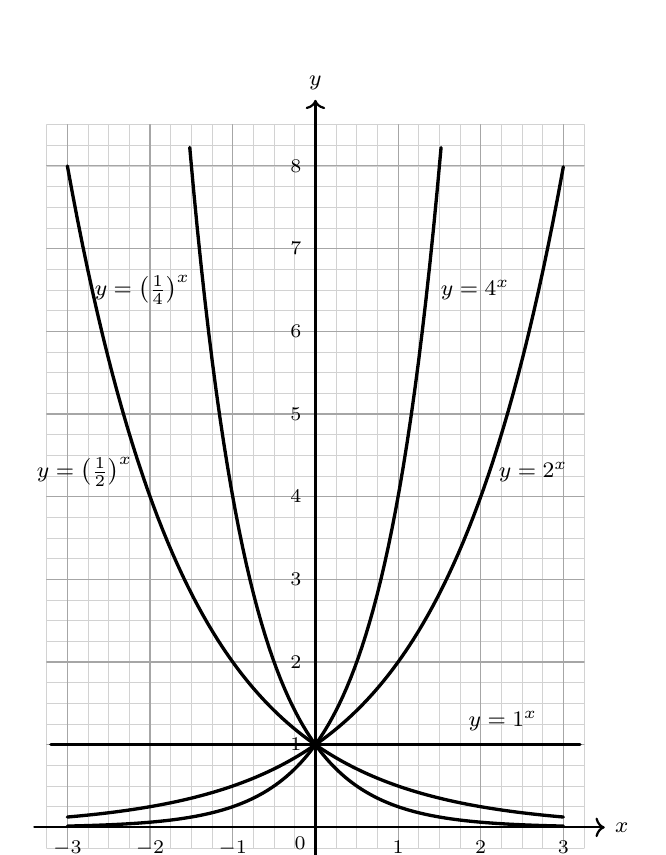
\begin{tikzpicture}[scale=1.05, line cap=round, line join=round]
    % Grid
    \draw[step=0.25cm, gray!35, very thin] (-3.25, -0.25) grid (3.25, 8.5);
    \draw[step=1cm, gray!70, thin] (-3.25, -0.25) grid (3.25, 8.5);

    % Axes
    \draw[thick, ->] (-3.4, 0) -- (3.5, 0) node[right, font=\footnotesize] {$x$};
    \draw[thick, ->] (0, -0.4) -- (0, 8.8) node[above, font=\footnotesize] {$y$};

    % Axis numbers
    \foreach \x in {-3, -2, -1, 1, 2, 3} {
        \node[below, font=\scriptsize] at (\x, -0.05) {$\x$};
    }
    \node[below left, font=\scriptsize] at (0, 0) {$0$};
    \foreach \y in {1, 2, 3, 4, 5, 6, 7, 8} {
        \node[left, font=\scriptsize] at (-0.05, \y) {$\y$};
    }

    % Curves
    % y = 4^x
    \draw[very thick, domain=-3:1.52, samples=100] plot (\x, {pow(4, \x)});
    \node[right, font=\footnotesize] at (1.4, 6.5) {$y=4^x$};

    % y = (1/4)^x
    \draw[very thick, domain=-1.52:3, samples=100] plot (\x, {pow(0.25, \x)});
    \node[left, font=\footnotesize] at (-1.4, 6.5) {$y=\left(\frac{1}{4}\right)^x$};

    % y = 2^x
    \draw[very thick, domain=-3:3, samples=100] plot (\x, {pow(2, \x)});
    \node[right, font=\footnotesize] at (2.1, 4.3) {$y=2^x$};

    % y = (1/2)^x
    \draw[very thick, domain=-3:3, samples=100] plot (\x, {pow(0.5, \x)});
    \node[left, font=\footnotesize] at (-2.1, 4.3) {$y=\left(\frac{1}{2}\right)^x$};

    % y = 1^x = 1
    \draw[very thick, domain=-3.2:3.2] plot (\x, 1);
    \node[above left, font=\footnotesize] at (2.8, 1.05) {$y=1^x$};
\end{tikzpicture}
\end{center}

\paragraph{【例 3】} $y = f(x) = (\sqrt{2})^{-x}$ 是一個絕對遞減函數. \\
因為由指數的基本性質及 $(\sqrt{2})^0 = 1$，我們有
\[
(\sqrt{2})^{-x} = \frac{1}{(\sqrt{2})^x}.
\]
由【例 2】知道 $(\sqrt{2})^x$ 是絕對遞增函數，所以 $(\sqrt{2})^{-x}$ 是絕對遞減函數.

\paragraph{【例 4】} $y = f(x) = \left(\frac{99}{100}\right)^x$ 是絕對遞減函數. \\
因為 $\frac{99}{100} < 1$，我們有
\[
f(1) < f(0).
\]

\subsection*{習題 4-4}

\begin{enumerate}
    \item 試寫出定理 2 遞減情形的詳細證明.
    \item 下面那些函數是遞增的？遞減的？絕對遞增的？絕對遞減的？
    \begin{enumerate}[(i)]
        \item $y = f(x) = x^3$.
        \item $y = f(x) = x^2$.
        \item $y = f(x) = x+5$.
        \item $y = f(x) = -x+7$.
        \item $y = f(x) = [x]$（高斯符號）.
    \end{enumerate}
    \item $y = f(x) = x^2$ 在什麼範圍是遞增的？在什麼範圍是遞減的？
    \item $y = f(x) = (x-1)^2+5$ 在什麼範圍是遞增的？在什麼範圍是遞減的？
    \item 如果 $f(x), g(x)$ 都是遞增的，$f(x)\cdot g(x)$ 是不是遞增的？請討論.
    \item 假設連續函數 $f(x)$ 對一切有理數 $x, y$，滿足 $f(x+y) = f(x)+f(y)$，那麼可以找到一個實數 $c$，使得 $f(x) = cx$.
\end{enumerate}

\subsection{對數函數}\label{sec:b2_4-3}

\subsubsection*{3-1 對數}

在前面我們引入了指數的概念，就是對於正實數 $a$ 與任意實數 $\alpha$，給予符號 $a^\alpha$ 明確的意義. 現在我們利用這種概念再介紹一個新的符號如下：

\begin{definition*}
給定一個不等於 1 的正實數 $a$，對於正實數 $b$，如果存在一個實數 $c$，滿足下列關係：
\[
a^c = b,
\]
我們就說 $c$ 是以 $a$ 為底，$b$ 的對數. 用符號
\[
\log_a b = c
\]
表示.
\end{definition*}

\noindent\textbf{【討論】}
\begin{enumerate}
    \item 由定義中的條件 $b = a^c$，$b$ 必須是一個正數. 所以對數只對於正實數定義，零或負數的對數沒有意義.
    \item 由於指數的性質，對於兩個實數 $c_1, c_2$，我們知道
    \[
    c_1 \neq c_2 \iff a^{c_1} \neq a^{c_2}.
    \]
    成立. 因此在定義中對應於 $b$ 的實數 $c$ 是唯一的，所以對數 $\log_a b$ 的定義是明確而有意義的（是一個確定的實數）.
    \item 因為對任意實數 $c,\; 1^c = 1$，在 $a^c = b$ 中，當 $a = 1$ 時，$b$ 非要等於 1 不可，而 $c$ 可以是任意的實數. 所以以 1 為底的對數沒有意義.
\end{enumerate}

\paragraph{【例 1】}
\begin{enumerate}[(i)]
    \item $10^2 = 100 \iff \log_{10} 100 = 2$.
    \item $3^5 = 243 \iff \log_3 243 = 5$.
    \item $4^{\frac{1}{4}} = \sqrt{2} \iff \log_4 \sqrt{2} = \frac{1}{4}$.
    \item $2^{10} = 1024 \iff \log_2 1024 = 10$.
    \item $12^2 = 144 \iff \log_{12} 144 = 2$.
    \item $3^{-1} = \frac{1}{3} \iff \log_3 \frac{1}{3} = -1$.
\end{enumerate}

由對數的定義，我們有下面的推論：

\begin{prop}[推論]
設 $a$ 是不等於 1 的正實數，$b$ 是任意正實數，$c$ 是任意實數，那麼我們有
\[
a^{\log_a b} = b, \quad \log_a(a^c) = c.
\]
\end{prop}

\paragraph{【例 2】}
\begin{enumerate}[(i)]
    \item $10^{\log_{10} 100} = 100,\quad \log_{10}(10^2) = 2$.
    \item $3^{\log_3 243} = 243,\quad \log_3(3^5) = 5$.
    \item $4^{\log_4 \sqrt{2}} = \sqrt{2},\quad \log_4(4^{\frac{1}{4}}) = \frac{1}{4}$.
    \item $2^{\log_2 1024} = 1024,\quad \log_2(2^{10}) = 10$.
    \item $12^{\log_{12} 144} = 144,\quad \log_{12}(12^2) = 2$.
    \item $3^{\log_3 \frac{1}{3}} = \frac{1}{3},\quad \log_3(3^{-1}) = -1$.
\end{enumerate}

依據這個推論，$c = \log_a b\; (a, b > 0,\; a \neq 1)$ 就是方程式
\begin{equation}
a^x - b = 0 \label{eq:b2-ch4-ax-minus-b}
\end{equation}
唯一的解. 事實上，對於任意正實數 $b$，\eqref{eq:b2-ch4-ax-minus-b} 式必定有解.

\begin{theorem}
給定不等於 1 的正實數 $a$，對於任意正實數 $b$，一定存在一個實數 $c$，滿足 \eqref{eq:b2-ch4-ax-minus-b} 式.
\end{theorem}
\noindent\textbf{【證明】} 假設 $a > 1$（$a < 1$ 時考慮 $a' = \frac{1}{a}$ 即可）. 分三種情形討論：
\begin{enumerate}[(i)]
    \item $b = 1$ 時，$c = 0,\; a^0 = 1$.
    \item $b > 1$ 時，我們先求出一個正整數 $k$，使得
    \[
    a^k > b.
    \]
    令 $a_1 = a-1,\; b_1 = b-1$，因 $a > 1, b > 1$，所以 $a_1, b_1$ 是兩個正實數. 由上一章 § 3，實數的阿基米德性質，我們知道存在一個正整數 $k$，使得
    \[
    k a_1 > b_1.
    \]
    兩邊同時加 1，得
    \[
    1 + k a_1 > 1 + b_1 = b.
    \]
    又因 $a_1 > 0$ 我們有
    \[
    a^k = (1+a_1)^k > 1 + k a_1 > 1 + b_1 = b,
    \]
    所以
    \[
    a^k > b.
    \]
    設函數 $y = f(x) = a^x$. 由假設 $b > 1$ 及以上導出的不等式，就有
    \[
    f(0) < b < f(k).
    \]
    現在由指數函數 $f$ 的連續性，以及連續函數的中間值定理知道，在 0 與 $k$ 之間有實數 $c$ 存在，滿足
    \[
    b = f(c) = a^c.
    \]
    \item $b < 1$ 時，仿照情形 (ii) 中的討論，我們可以求出正整數 $k$，使得 $a^k > \frac{1}{b} > 1$. 所以
    \[
    a^{-k} < b < a^0 = 1.
    \]
    同理在 $-k$ 與 0 之間存在實數 $c$，滿足
    \[
    b = f(c) = a^c.
    \]
\end{enumerate}
\hfill〔定理 3 證畢〕

\paragraph{【例 3】}
\begin{enumerate}[(i)]
    \item $2^x - 50 = 0$ 的解 $x$ 在 5 與 6 之間. \\
    因為 $2^5 = 32 < 50 < 2^6 = 64$.
    \item $\left(\frac{15}{10}\right)^x - 2 = 0$ 的解 $x$ 在 1 與 2 之間. \\
    因為 $\frac{15}{10} < 2 < \left(\frac{15}{10}\right)^2 = \frac{225}{100}$.
\end{enumerate}

\subsection*{習題 4-5}

\begin{enumerate}
    \item 計算下列各對數之值：
    \begin{enumerate}[(i)]
        \item $\log_4 8$.
        \item $\log_9(\sqrt[3]{3})$.
        \item $\log_8(32^2)$.
        \item $\log_{10}(100^{\frac{1}{3}})$.
        \item $\log 1000^{\frac{1}{10}}$\phantomsection\label{note:b2-ch4-p98-log-base}.
        \item $\log_2(\log_2 16)$.
    \end{enumerate}
    \item 化簡：
    \begin{enumerate}[(i)]
        \item $2^{\log_2 5}$.
        \item $2^{-\log_3 2}$.
        \item $\log_2(2^5)$.
        \item $\log_{10}(10^3)$.
        \item $\log_2(\log_{10} 100)$.
    \end{enumerate}
    \item 化簡下列各式：
    \begin{enumerate}[(i)]
        \item $2^{2\log_2 x}$.
        \item $2^{\log_2 x + \log_2 y}$.
        \item $2^{-\log_2 x}$.
        \item $2^{\log_2 2x - \log_2 y}$.
        \item $2^{2\log_2 x - \log_2 y}$.
    \end{enumerate}
    \item 化簡下列各式：
    \begin{enumerate}[(i)]
        \item $\log_2(4^x)$.
        \item $\log_2(a^{\log_a x})$.
        \item $\log_2(4^x \cdot 2^y)$.
        \item $\log_2(\sqrt{2}\cdot 2^x)$.
    \end{enumerate}
    \item 下列各方程式的解，各在那兩個相鄰的整數之間？
    \begin{enumerate}[(i)]
        \item $2^x - 5 = 0$.
        \item $2^x - \frac{1}{10} = 0$.
        \item $3^x - \frac{1}{10} = 0$.
        \item $2^x - 1000 = 0$.
        \item $3^x - \frac{1}{250} = 0$.
    \end{enumerate}
    \item 
    \begin{enumerate}[(i)]
        \item 試證 $\log_{10} 3$ 不是有理數.
        \item 討論一般的情形，即對於大於 1 的正整數 $a, b$，在什麼情形之下 $\log_a b$ 不是有理數？
    \end{enumerate}
\end{enumerate}

\subsubsection*{3-2 對數的基本特性}

顯然對數的性質與指數的性質間具有密切關係：譬如對應於指數定則 (1), (2)，就有下述對數定則：
\begin{align}
\log_a(uv) &= \log_a u + \log_a v \tag{I}\label{eq:b2-ch4-log-rule-prod} \\
\log_a w &= \log_a c \cdot \log_c w \tag{II}\label{eq:b2-ch4-log-rule-base}
\end{align}
其中 $a, c$ 是不等於 1 的正實數，$u, v, w$ 是任意正實數，\eqref{eq:b2-ch4-log-rule-base} 式又叫做對數換底公式.

\noindent\textbf{【證明】} \eqref{eq:b2-ch4-log-rule-prod} 式的證明留作習題，現在證明 \eqref{eq:b2-ch4-log-rule-base} 式如下：\\
由定理 3 我們可以找到兩個實數 $\alpha, \beta$，使得
\[
c = a^\alpha,\quad w = c^\beta \quad (\text{或 } \alpha = \log_a c,\; \beta = \log_c w).
\]
因此
\[
w = (a^\alpha)^\beta = a^{\alpha\beta}.
\]
所以
\[
\log_a w = \log_a a^{\alpha\beta} = \alpha\beta = \log_a c \cdot \log_c w.
\]
\hfill〔證畢〕

與指數的性質相仿，對數也有下列性質：（$a$ 為正實數）
\begin{equation}
\begin{cases}
\text{如 } a > 1, & \text{則 } b > c \implies \log_a b > \log_a c \\
\text{如 } a < 1, & \text{則 } b > c \implies \log_a b < \log_a c
\end{cases} \tag{III}\label{eq:b2-ch4-log-mono}
\end{equation}

\paragraph{【例 4】} $\log_a u^\alpha = \alpha\log_a u$（$a$ 是不等於 1 的正實數，$u$ 是正實數，$\alpha$ 是任意實數）. \\
\noindent\textbf{【證明】} 設 $\log_a u = b$，就有 $a^b = u$，所以
\[
(a^b)^\alpha = a^{\alpha b} = u^\alpha,
\]
又由對數的定義得到
\[
\log_a u^\alpha = \alpha b = \alpha\log_a u.
\]

\paragraph{【例 5】} $\log_a c = (\log_c a)^{-1}$（$a, c$ 是不等於 1 的正實數）. \\
\noindent\textbf{【證明】} 在公式 \eqref{eq:b2-ch4-log-rule-base} 中，令 $w = a$.

\paragraph{【例 6】} 已知 $\log_{10} 2 = 0.3010$，求 $\log_{10} 5, \log_{10} 40, \log_2 5$. \\
\noindent\textbf{【解】}
\begin{align*}
\log_{10} 5 &= \log_{10} \frac{10}{2} = \log_{10} 10 - \log_{10} 2 \\
&= 1 - 0.3010 = 0.6990. \\
\log_{10} 40 &= \log_{10}(2)^2 + \log_{10} 10 = 2\log_{10} 2 + 1 \\
&= 2\cdot(0.3010) + 1 = 1.6020. \\
\log_2 5 &= \log_2 \frac{10}{2} = \log_2 10 - \log_2 2 \\
&= (\log_{10} 2)^{-1} - 1 = \frac{1}{0.3010} - 1 = \frac{699}{301}.
\end{align*}

\subsection*{習題 4-6}

\begin{enumerate}
    \item 證明對數定則 (I).
    \item 證明 $\log_a \frac{u}{v} = \log_a u - \log_a v$（其中 $a$ 是不等於 1 的正實數，$u, v$ 是任意正實數）.
    \item 證明 $\log_a b \cdot \log_b a = 1$（其中 $a, b$ 是不等於 1 的正實數）.
    \item 下面那些式子是錯的？
    \begin{enumerate}[(i)]
        \item $\log_2(-5) = -\log_2 5$.
        \item $\log_2(3\cdot 5) = \log_2 3 \cdot \log_2 5$.
        \item $\log_2 8 + \log_{\frac{1}{2}} 8 = 0$.
        \item $\log_2(5^3) = (\log_2 5)^3$.
        \item $\log_2(5+3) = \log_2 5 + \log_2 3$.
        \item $\log_2 10 = (\log_{\frac{1}{2}} 10)^{-1}$.
    \end{enumerate}
    \item 求下列各式之值：
    \begin{enumerate}[(i)]
        \item $\frac{1}{2}\log_3 9$.
        \item $\log_4 2 + \log_4 8$.
        \item $3\log_{10} 2 - \log_{10} 80$.
        \item $\log_5 10 - \log_5 \frac{2}{\sqrt{5}}$.
    \end{enumerate}
    \item 令 $\log_2 x = X,\; \log_2 y = Y$，將下列各式以 $X, Y$ 表示：
    \begin{enumerate}[(i)]
        \item $\log_2 xy^2$.
        \item $\log_2 \sqrt{xy}$.
        \item $\log_2 \sqrt{x^3 y}$.
        \item $\log_2 \sqrt[3]{x^5 y^2}$.
    \end{enumerate}
    \item 改正下式右邊的錯誤：
    \[
    \log_2 \sqrt{15} = \frac{1}{2}\log_2 3 + \log_2 5.
    \]
    \item 計算 $\log_2 13 + \frac{1}{2}\log_2 25 + \log_2 \frac{4}{7} - \log_2 \frac{13}{35}$.
    \item $(\log_2 3 + \log_4 9)(\log_3 4 + \log_9 2) = {?}$
    \item $\log_a b \cdot \log_b c \cdot \log_c a = {?}$（$a, b, c$ 是不等於 1 的正數.）
\end{enumerate}

\subsubsection*{3-3 對數函數}

根據前面的定理 3，我們知道，如果 $a$ 是一個不等於 1 的正實數，對數 $\log_a b$ 對於任意正實數 $b$ 都有明確的意義. 所以當我們用變數 $x$ 表示一個任意正實數時，$y = f(x) = \log_a x$ 就是一個函數，通常叫做以 $a$ 為底的對數函數.

由定義，對數函數與指數函數有下列關係：
\[
y = \log_a x \iff x = a^y.
\]
由對數的性質，我們直接得到對數函數的性質：
\begin{enumerate}[(i)]
    \item $f(\alpha\beta) = f(\alpha) + f(\beta)$;
    \item $\begin{cases} \text{若 } a > 1, & \text{則 } \alpha > \beta \implies f(\alpha) > f(\beta) \text{（絕對單調遞增）}. \\ \text{若 } a < 1, & \text{則 } \alpha > \beta \implies f(\alpha) < f(\beta) \text{（絕對單調遞減）}. \end{cases}$
\end{enumerate}
對於所有正實數 $\alpha, \beta$ 都成立. 反之，任意滿足性質 (i) 的絕對單調函數必定是一個對數函數.

\begin{theorem}
如果 $y = f(x)$ 是一個絕對單調函數而且滿足上述性質 (i)，那麼它一定是一個對數函數. 我們可以找到一個適當正實數 $a \neq 1$，使得
\[
f(x) = \log_a x.
\]
\end{theorem}
\noindent\textbf{【證明】} 證明方法與定理 2 相似，請同學們比照研讀. 我們考慮單調遞增的情形. 由性質 (i) 得到
\[
f(v) = f(1\cdot v) = f(1) + f(v) \implies f(1) = 0.
\]
令 $f(2) = c$，由單調遞增性（即 (ii)）有
\[
c = f(2) > f(1) = 0.
\]
又由 (i) 得
\begin{align*}
f(2^n) &= \underbrace{f(2) + \dots\dots + f(2)}_{n \text{ 項}} = n\cdot f(2) = nc,\quad n \in \mathbb{N}. \\
m\cdot f(2^{\frac{1}{m}}) &= f((\sqrt[m]{2})^m) = f(2) = c. \\
\implies f(2^{\frac{1}{m}}) &= \frac{1}{m}\cdot c,\quad m \in \mathbb{N}. \\
\implies f(2^{\frac{n}{m}}) &= \frac{n}{m}\cdot c,\quad m, n \in \mathbb{N}.
\end{align*}
又
\[
f(2^{-r}) + f(2^r) = f(2^{-r}\cdot 2^r) = f(1) = 0 \implies f(2^{-r}) = -rc \quad (r \in \mathbb{Q}).
\]
所以對於所有有理數 $r \in \mathbb{Q},\; f(2^r) = rc$. 從此不難用單調性和極限過程導出
\[
f(2^\beta) = \beta\cdot c
\]
對於所有實數 $\beta \in \mathbb{R}$ 都成立. \\
令 $a = 2^{\frac{1}{c}} > 1$，則有
\begin{align*}
f(a) &= f(2^{\frac{1}{c}}) = \frac{1}{c}\cdot c = 1; \\
f(a^u) &= f((2^{\frac{1}{c}})^u) = f(2^{\frac{u}{c}}) = \frac{u}{c}\cdot c = u.
\end{align*}
但是 $x = a^{\log_a x}$，代入上式就得到
\[
f(x) = f(a^{\log_a x}) = \log_a x.
\]
\hfill〔定理 4 證畢〕\\
單調遞減的情形留作習題.

\paragraph{【例 7】} 設 $a$ 是一個不等於 1 的正實數，則函數 $f(x) = \log_a x$ 與 $g(x) = \log_{\frac{1}{a}} x$ 滿足下列關係：
\[
f(x) = -g(x).
\]
\noindent\textbf{【證明】} 利用 (3-2) 中對數換底公式 (II)，我們有
\[
\log_a x = \log_a \frac{1}{a} \cdot \log_{\frac{1}{a}} x.
\]
但 $\log_a \frac{1}{a} = -1$，所以 $\log_a x = -\log_{\frac{1}{a}} x$，即
\[
f(x) = -g(x).
\]

下圖中作出對數函數 $y = \log_2 x$ 與 $y = \log_{\frac{1}{2}} x$ 的圖形，我們可以看出它們的單調性，以及這種關於 $x$ 軸的對稱關係.

\begin{center}
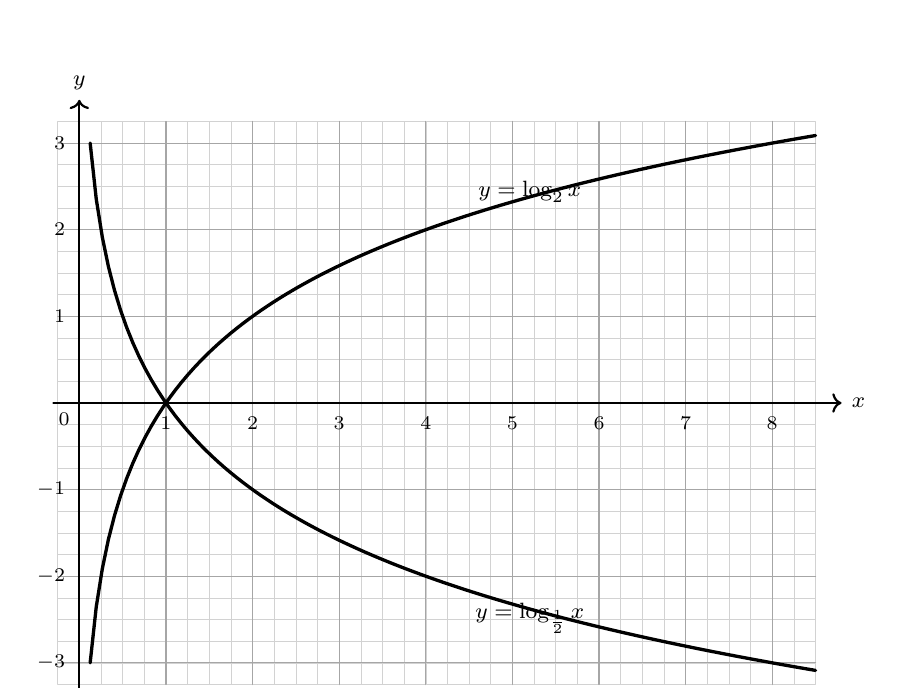
\begin{tikzpicture}[scale=1.1, line cap=round, line join=round]
    % Grid
    \draw[step=0.25cm, gray!35, very thin] (-0.25, -3.25) grid (8.5, 3.25);
    \draw[step=1cm, gray!70, thin] (-0.25, -3.25) grid (8.5, 3.25);

    % Axes
    \draw[thick, ->] (-0.3, 0) -- (8.8, 0) node[right, font=\footnotesize] {$x$};
    \draw[thick, ->] (0, -3.4) -- (0, 3.5) node[above, font=\footnotesize] {$y$};

    % Axis numbers
    \foreach \x in {1, 2, 3, 4, 5, 6, 7, 8} {
        \node[below, font=\scriptsize] at (\x, -0.05) {$\x$};
    }
    \node[below left, font=\scriptsize] at (0, 0) {$0$};
    \foreach \y in {-3, -2, -1, 1, 2, 3} {
        \node[left, font=\scriptsize] at (-0.05, \y) {$\y$};
    }

    % Curves
    % y = log_2(x)
    \draw[very thick, domain=0.125:8.5, samples=120] plot (\x, {ln(\x)/ln(2)});
    \node[above, font=\footnotesize] at (5.2, 2.2) {$y=\log_2 x$};

    % y = log_{1/2}(x)
    \draw[very thick, domain=0.125:8.5, samples=120] plot (\x, {-ln(\x)/ln(2)});
    \node[below, font=\footnotesize] at (5.2, -2.2) {$y=\log_{\frac{1}{2}} x$};
\end{tikzpicture}
\end{center}

\subsection*{習題 4-7}

\begin{enumerate}
    \item 已知正數 $x, y$，的和是 8，那麼 $\log_2 x + \log_2 y$ 的最大值是多少？
    \item 當 $2x+5y=20$ 時，試求 $\log_2 x + \log_2 y$ 之最大值.
    \item 設 $x > 2, y > 2$，比較下列各式之大小：
    \[
    \log_2 \frac{x+y}{2}, \quad \frac{1}{2}\log_2(x+y), \quad \frac{1}{2}(\log_2 x + \log_2 y).
    \]
    \item 滿足下列不等式之整數有幾個？
    \[
    0 \le \log_3(\log_3 x) < 1.
    \]
    \item 設 $x > 1, y > 1$，且 $2\log_x y - 2\log_y x + 3 = 0$. 那麼 $x^2 - 4y^2$ 的最小值是多少？
    \item 設 $a > 1, b > 1$，試證
    \[
    \log_a b + \log_b a \ge 2.
    \]
    \item 解 $\log_3 x = -2$.
    \item 解 $\log_x 10 = -1$.
    \item 解 $2 = \log_x \frac{1}{4}$.
    \item 解 $\log_{10}(x+1) + \log_{10}(x-2) = 1$.
    \item 解 $\frac{1}{2}\log_{10} 2 + \log_{10} \sqrt{x} = \log_{10}(1+\frac{x}{2})$.
    \item 解
    \[
    \begin{cases}
    \log x + \log y = 2, \\
    x^2 + y^2 = 425.
    \end{cases}
    \]
    \item 解下列各指數方程式：
    \begin{enumerate}[(i)]
        \item $2^x = 3^{x-1}$.
        \item $4.5^{x-1} = 10^{x+1}$.
        \item $7.6^{2x} = 11^{x+3}$.
    \end{enumerate}
\end{enumerate}

\subsection{反函數}\label{sec:b2_4-4}

設 $y = f(x)$ 是由數集 $A$ 到數集 $B$ 的函數，如果對於 $A$ 中任意不同的 $\alpha, \beta$，它們在 $B$ 中的對應數 $f(\alpha), f(\beta)$ 也不相同：
\[
\alpha, \beta \in A,\quad \alpha \neq \beta \implies f(\alpha) \neq f(\beta).
\]
我們就說 $f$ 是嵌射的 (injective) 函數，或者說 $f$ 是個嵌射 (injection).

\paragraph{【例 1】} 恆等函數 $y = f(x) = x,\; (f: A \to A \text{（其中 $A$ 為任意數集））}$ 是嵌射的.

\paragraph{【例 2】} 線性函數 $y = f(x) = ax+b\; (a\neq 0),\; f: \mathbb{R} \to \mathbb{R}$ 也是嵌射的.

\paragraph{【例 3】} $y = f(x) = x^2,\; f: \mathbb{R} \to \mathbb{R}$ 不是嵌射的（為什麼？），但是 $f: \mathbb{R}^+ \to \mathbb{R}^+$ 是嵌射的，其中 $\mathbb{R}^+$ 是所有正實數的集合.

由絕對單調的意義，絕對單調函數是嵌射的，所以指數函數與對數函數都是嵌射的.

\subsection*{習題 4-8}

下列函數各在那些範圍是嵌射的？
\begin{enumerate}
    \item $y = f(x) = x^3$.
    \item $y = f(x) = x^n,\; n$ 是正整數.
    \item $y = f(x) = \sqrt{x}$.
    \item $y = f(x) = |x|$.
    \item $y = f(x) = [x]$（高斯符號）.
    \item $y = f(x) = \log_2 x^2$.
\end{enumerate}

我們現在來討論函數的另一種性質. 考慮由 $A$ 到 $B$ 的函數 $y = f(x)$，如果 $B$ 中每一個數 $b$ 在函數 $f$ 的作用下，都是 $A$ 中某一個數或某些數的對應數；也就是說：
\[
\text{對於任意 } b \in B\text{，存在至少一個 } a \in A\text{，使得 } b = f(a).
\]
這樣我們就說：$f$ 是由 $A$ 到 $B$ 的蓋射 (surjcetion)\phantomsection\label{note:b2-ch4-p106-surjcetion} 或 $f$ 是個由 $A$ 到 $B$ 的蓋射的 (surjective) 函數.

由 $A$ 到 $B$ 的一個函數 $y = f(x)$，如果同時又是蓋射的，又是嵌射的，就叫對射的 (bijective)，或者 $f$ 叫做一個由 $A$ 到 $B$ 的對射 (bijection).

\paragraph{【例 4】} 例一、例二中的恆等函數與線性函數都是由 $\mathbb{R}$ 到 $\mathbb{R}$ 的對射.

\paragraph{【例 5】} 指數函數是由 $\mathbb{R}$ 到 $\mathbb{R}$ 的嵌射而不是蓋射，所以也不是對射的. 而對數是由 $\mathbb{R}^+$ 到 $\mathbb{R}$ 的對射.

\paragraph{【例 6】} 但指數函數是由 $\mathbb{R}$ 到 $\mathbb{R}^+$（正實數的集合）的對射. 由此可知嵌射，對射，蓋射等觀念和集 $A, B$ 有關.

\begin{theorem}
如果 $f$ 是由數集 $A$ 到數集 $B$ 的對射，那麼必存在一個唯一的由 $B$ 到 $A$ 的對射 $g$，使得
\[
f(a) = b \iff g(b) = a,\quad (a \in A, b \in B).
\]
也就是說
\[
f(g(b)) = b,\quad g(f(a)) = a.
\]
\end{theorem}

\begin{definition*}
上面定理中的函數 $g$ 叫做 $f$ 的反函數（或逆函數），用符號 $f^{-1}$ 表示，不難看出 $f$ 也是 $g$ 的反函數. 所以 $f$ 與 $g$ 互為反函數.
\[
(g = f^{-1},\; f = g^{-1} = (f^{-1})^{-1}).
\]
\end{definition*}

\noindent\textbf{【證明】（定理 5）} 對於任意 $b \in B$，由 $f$ 的蓋射性質，知道存在至少一個 $a \in A$，使得 $f(a) = b$，而且由於 $f$ 的嵌射性質，知道這樣的 $a$ 最多只有一個. 因此我們很自然的可以作一個由 $B$ 到 $A$ 的對應：$b \longrightarrow a$，這樣的對應很顯然的是一個由 $B$ 到 $A$ 的函數，這就是我們所要求的函數 $g$. \\
$g$ 是嵌射的，因為對於 $b_1, b_2 \in B$，
\[
g(b_1) = g(b_2) = a \in A \implies f(a) = b_1,\; f(a) = b_2 \implies b_1 = b_2.
\]
$g$ 是蓋射的，因為對於任意 $a \in A,\; f(a) = b \in B$，就有
\[
g(b) = a.
\]

\paragraph{【例 7】} 恆等函數 $f: A \to A$ 的反函數 $f^{-1} = f$.

\paragraph{【例 8】} 線性函數 $f(x) = ax+b\; (a\neq 0)$ 的反函數是
\[
f^{-1}(x) = \frac{1}{a}x - \frac{b}{a}.
\]
辦法很簡單，我們由 $y = ax+b,\; a\neq 0$ 來反解 $x$，得到
\[
x = \frac{1}{a}y - \frac{b}{a},\quad \text{並把它寫做 } f^{-1}(y). \text{ 所以}
\]
\[
f^{-1}(x) = \frac{1}{a}x - \frac{b}{a}.
\]

\begin{prop}[推論 1]
如果 $f$ 是由數集 $A$ 到數集 $B$ 的絕對遞增（遞減）蓋射的函數，那麼反函數 $f^{-1}$ 存在，而且是由 $B$ 到 $A$ 的絕對遞增（遞減）蓋射的函數.
\end{prop}
\noindent\textbf{【證明】} 由上面定理，知道反函數 $f^{-1}$ 存在，而且是一個由 $B$ 到 $A$ 的對射，對於 $f^{-1}$ 的絕對單調性，我們不妨假設 $f$ 是遞增的. \\
如果 $b_1, b_2 \in B$，而且 $b_1 < b_2$，設 $a_1 = f^{-1}(b_1),\; a_2 = f^{-1}(b_2)$，那麼 $f(a_1) = b_1,\; f(a_2) = b_2$，如果 $a_1 \ge a_2$，由 $f$ 的絕對遞增性質，知道 $b_1 = f(a_1) \ge f(a_2) = b_2$，與 $b_1 < b_2$ 的假設矛盾，因此 $a_1 < a_2$，即
\[
b_1 < b_2 \implies f^{-1}(b_1) < f^{-1}(b_2).
\]

\begin{prop}[推論 2]
設 $a$ 為不等於 1 的正實數，則以 $a$ 為底的指數函數 $y = f(x) = a^x,\; f: \mathbb{R} \to \mathbb{R}^+$（正實數的集合），與對數函數 $x = g(y) = \log_a y,\; g: \mathbb{R}^+ \to \mathbb{R}$ 互為反函數.
\end{prop}

\begin{theorem}
如果 $f$ 是一個由區間 $[a, b]$ 到區間 $[c, d]$ 的對射的連續函數，那麼 $f$ 是絕對單調函數.
\end{theorem}
\noindent\textbf{【證明】} 不妨假設 $f(a) < f(b)$，我們要證明 $f$ 是絕對遞增. 對於 $(a, b)$ 中任意數 $a_1$，如果
\[
f(a_1) < f(a) < f(b),
\]
那麼由 $f$ 在區間 $[a, b]$ 上的連續性與連續函數的中間值定理，在 $(a_1, b)$ 中必定存在一個數 $b_1$，使得
\[
f(b_1) = f(a).
\]
這和 $f$ 的嵌射性質不合，又如果 $f(a) < f(b) < f(a_1)$，那麼在 $(a, a_1)$ 中必定存在一個數 $b_2$，使得
\[
f(b_2) = f(b).
\]
又得到矛盾，所以
\[
f(a) < f(a_1) < f(b).
\]
現在對於任意兩數 $a_1, a_2;\; a < a_1 < a_2 < b$，由以上的討論，我們知道 $f(a) < f(a_2)$. 把 $a_2$ 代替上面的討論中的 $b$，就得到 $f(a) < f(a_1) < f(a_2)$. 綜合以上結果：
\[
a \le a_1 < a_2 \le b \implies f(a_1) < f(a_2).
\]
在這種情形下，顯然 $f(a) = c,\; f(b) = d$，當然在遞減的情形，就有 $f(a) = d,\; f(b) = c$.

\begin{theorem}
在定理 6 的假設下，$f$ 的反函數 $f^{-1}$ 存在，而且也是連續的.
\end{theorem}
\noindent\textbf{【證明】} 如果 $f$ 是絕對遞增的，由推論 1 知道 $f^{-1}$ 存在而且是絕對遞增的. 設 $y_0$ 是 $c, d$ 之間的一個任意數，任意選取一個遞增，一個遞減的數列 $\langle y_n \rangle, \langle y'_n \rangle$ 逼近 $y_0$.
\[
y_1 < y_2 < \dots\dots < y_n < \dots\dots < y_0 < \dots\dots < y'_n < \dots\dots < y'_2 < y'_1.
\]
並且
\[
y_0 = \lim_{n\to\infty} y_n = \lim_{n\to\infty} y'_n,\quad \lim_{n\to\infty}(y'_n - y_n) = 0.
\]
設 $x_0 = f^{-1}(y_0),\; x_n = f^{-1}(y_n),\; x'_n = f^{-1}(y'_n),\; n=1, 2, 3, \dots$，由 $f^{-1}$ 的單調遞增性得到
\[
x_1 < x_2 < \dots\dots < x_n < \dots\dots < x_0 < \dots\dots < x'_n < \dots\dots < x'_2 < x'_1.
\]
我們只要證明 $\lim_{n\to\infty}(x'_n - x_n) = 0$，也就是說
\[
\lim_{n\to\infty} x_n = x_0 = \lim_{n\to\infty} x'_n.
\]
如果不然，假設 $\lim_{n\to\infty} x_n \neq x_0$，那麼一定存在一個數 $a_1$：
\[
x_n < a_1 < x_0,\quad x = 1, 2, 3, \dots\dots\phantomsection\label{note:b2-ch4-p109-index-x}
\]
由函數 $f$ 的單調遞增性得到
\[
y_n < c_1 = f(a_1) < y_0,\quad n=1, 2, 3, \dots\dots
\]
但是這和 $\lim_{n\to\infty} y_n = y_0$ 互相矛盾，因此 $\lim_{n\to\infty} x_n = x_0$；\\
同理可證 $\lim_{n\to\infty} x'_n = x_0$.

由指數函數的連續性與定理 7，我們得到下面的推論.

\begin{prop}[推論]
對數函數 $y = f(x) = \log_a x$（$a$ 是一個不等於 1 的正實數）是連續函數.
\end{prop}

\subsection*{習題 4-9}

\begin{enumerate}
    \item 設 $f(x) = 2x-3, g(x) = x-1$ 為兩個多項式函數.
    \begin{enumerate}[(i)]
        \item 試求 $g[f(x)]$（這叫做函數 $f$ 與 $g$ 的合成函數，通常用符號 $g\circ f(x)$ 表示，亦即 $g\circ f(x) = g[f(x)]$）.
        \item 試證 $f$ 與 $g$ 都是對射，並求其反函數 $f^{-1}$ 與 $g^{-1}$.
    \end{enumerate}
    \item 設 $f(x) = \frac{1}{2}(a^x + a^{-x}),\; g(x) = \frac{1}{2}(a^x - a^{-x})$. \\
    試證 $f(x+y) = f(x)f(y) + g(x)g(y)$.
    \item 求函數 $y = \log_2(x-2)$ 的反函數.
    \item 求函數 $y = \log_2 \frac{1}{x}$ 的反函數.
    \item 求函數 $y = 2^{-2x}$ 的反函數.
    \item 對於下列各函數，分別找出最大的實數集合 $A, B$，使得函數 $f$ 成為自 $A$ 到 $B$ 的對射：
    \begin{enumerate}[(i)]
        \item $y = f(x) = x^2$.
        \item $y = f(x) = \sqrt{2x+1}$.
        \item $y = f(x) = x^3$.
        \item $y = f(x) = \log_2 |x|$.
        \item $y = f(x) = \log_2(1+x^2)$.
        \item $y = f(x) = 2^{1+2x}$.
        \item $y = f(x) = 2^{-|x|}$.
    \end{enumerate}
\end{enumerate}


\end{document}
